\begin{table}[H]
  \centering
  \begin{tabular}{|c|l|l|} \hline
    モジュール名                & \multicolumn{2}{l|}{home.dart}                                                                                                                   \\ \hline
    モジュール概要               & \multicolumn{2}{p{12cm}|}{ホーム画面を作成するモジュール}                                                                                                       \\ \hline
    責任者                   & \multicolumn{2}{l|}{新谷光城}                                                                                                                        \\ \hline
    \multirow{7}{*}{構成要素} & クラス名                                                                                & HomeRouterPage                                             \\ \cline{2-3}
                          & クラス種類                                                                               & extends AppRouter                                          \\ \cline{2-3}
                          & 処理概要                                                                                & \multicolumn{1}{p{12cm}|}{HomeをアクセスするためのRouter}            \\ \cline{2-3}
                          & 入力                                                                                  & なし                                                         \\ \cline{2-3}
                          & 出力                                                                                  & Route                                                      \\ \cline{2-3}
                          & \multicolumn{2}{l|}{他クラス・関数との関係}                                                                                                                 \\ \cline{2-3}
                          & \multicolumn{2}{p{14cm}|}{なし}                                                                                                                    \\ \hline
    \multirow{7}{*}{構成要素} & クラス名                                                                                & Home                                                       \\ \cline{2-3}
                          & クラス種類                                                                               & extends StatelessWidget                                    \\ \cline{2-3}
                          & 処理概要                                                                                & \multicolumn{1}{p{12cm}|}{ホーム画面のWidgetを動的に変更するクラス}         \\ \cline{2-3}
                          & 入力                                                                                  & なし                                                         \\ \cline{2-3}
                          & 出力                                                                                  & Widget                                                     \\ \cline{2-3}
                          & \multicolumn{2}{l|}{他クラス・関数との関係}                                                                                                                 \\ \cline{2-3}
                          & \multicolumn{2}{p{14cm}|}{home.dartのHomeStateクラスを組み込む}                                                                                           \\ \hline
    \multirow{7}{*}{構成要素} & クラス名                                                                                & HomeState                                                  \\ \cline{2-3}
                          & クラス種類                                                                               & extends StatelessWidget                                    \\ \cline{2-3}
                          & 処理概要                                                                                & \multicolumn{1}{p{12cm}|}{ホーム画面の状態を返すクラス}                  \\ \cline{2-3}
                          & 入力                                                                                  & なし                                                         \\ \cline{2-3}
                          & 出力                                                                                  & State                                                      \\ \cline{2-3}
                          & \multicolumn{2}{l|}{他クラス・関数との関係}                                                                                                                 \\ \cline{2-3}
                          & \multicolumn{2}{p{14cm}|}{
      home.dartのMainAppBarクラスを組み込む
      \newline change\_general\_corporation.dartのChangeGeneralCorporationプロバイダを組み込む
      \newline else\_list.dartのElseListクラスを呼び出すことで閲覧履歴画面を表示
    \newline post\_list.dartのPostListクラスを呼び出すことで閲覧履歴詳細画面を表示}                                                                                                                 \\ \hline
    \multirow{7}{*}{構成要素} & クラス名                                                                                & MainAppBar                                                 \\ \cline{2-3}
                          & クラス種類                                                                               & extends StatelessWidget, imprements PreferredSizeWidget    \\ \cline{2-3}
                          & 処理概要                                                                                & \multicolumn{1}{p{12cm}|}{ホーム画面用に作成を行ったAppBarを生成するコンポーネント} \\ \cline{2-3}
                          & 入力                                                                                  & Widget component                                           \\ \cline{2-3}
                          & 出力                                                                                  & Widget                                                     \\ \cline{2-3}
                          & \multicolumn{2}{l|}{他クラス・関数との関係}                                                                                                                 \\ \cline{2-3}
                          & \multicolumn{2}{p{14cm}|}{notice.dartのNoticeクラスを呼び出し通知画面を表示}                                                                                     \\ \hline
    \multirow{7}{*}{構成要素} & クラス名                                                                                & GeneralHomeButton                                          \\ \cline{2-3}
                          & クラス種類                                                                               & extends StatelessWidget                                    \\ \cline{2-3}
                          & 処理概要                                                                                & \multicolumn{1}{p{12cm}|}{一般利用者用画面でのボタンを生成するコンポーネント}       \\ \cline{2-3}
                          & 入力                                                                                  & なし                                                         \\ \cline{2-3}
                          & 出力                                                                                  & Widget                                                     \\ \cline{2-3}
                          & \multicolumn{2}{l|}{他クラス・関数との関係}                                                                                                                 \\ \cline{2-3}
                          & \multicolumn{2}{p{14cm}|}{else\_list.dartのElseListクラスを呼び出すことで応募履歴一覧画面、お気に入り一覧画面を表示}                                                              \\
    \hline
    \multirow{7}{*}{構成要素} & クラス名                                                                                & CompanyHomeButton                                          \\ \cline{2-3}
                          & クラス種類                                                                               & extends StatelessWidget                                    \\ \cline{2-3}
                          & 処理概要                                                                                & \multicolumn{1}{p{12cm}|}{法人利用者用画面でのボタンを生成するコンポーネント}       \\ \cline{2-3}
                          & 入力                                                                                  & なし                                                         \\ \cline{2-3}
                          & 出力                                                                                  & Widget                                                     \\ \cline{2-3}
                          & \multicolumn{2}{l|}{他クラス・関数との関係}                                                                                                                 \\ \cline{2-3}
                          & \multicolumn{2}{p{14cm}|}{
      else\_list.dartのElseListクラスを呼び出すことで応募履歴一覧画面、お気に入り一覧画面を表示
    \newline posted\_list.dartのPostedListクラスを呼び出すことで投稿広告一覧画面を表示}                                                                                                             \\ \hline
  \end{tabular}
\end{table}

\begin{figure}[H]
  \centering
  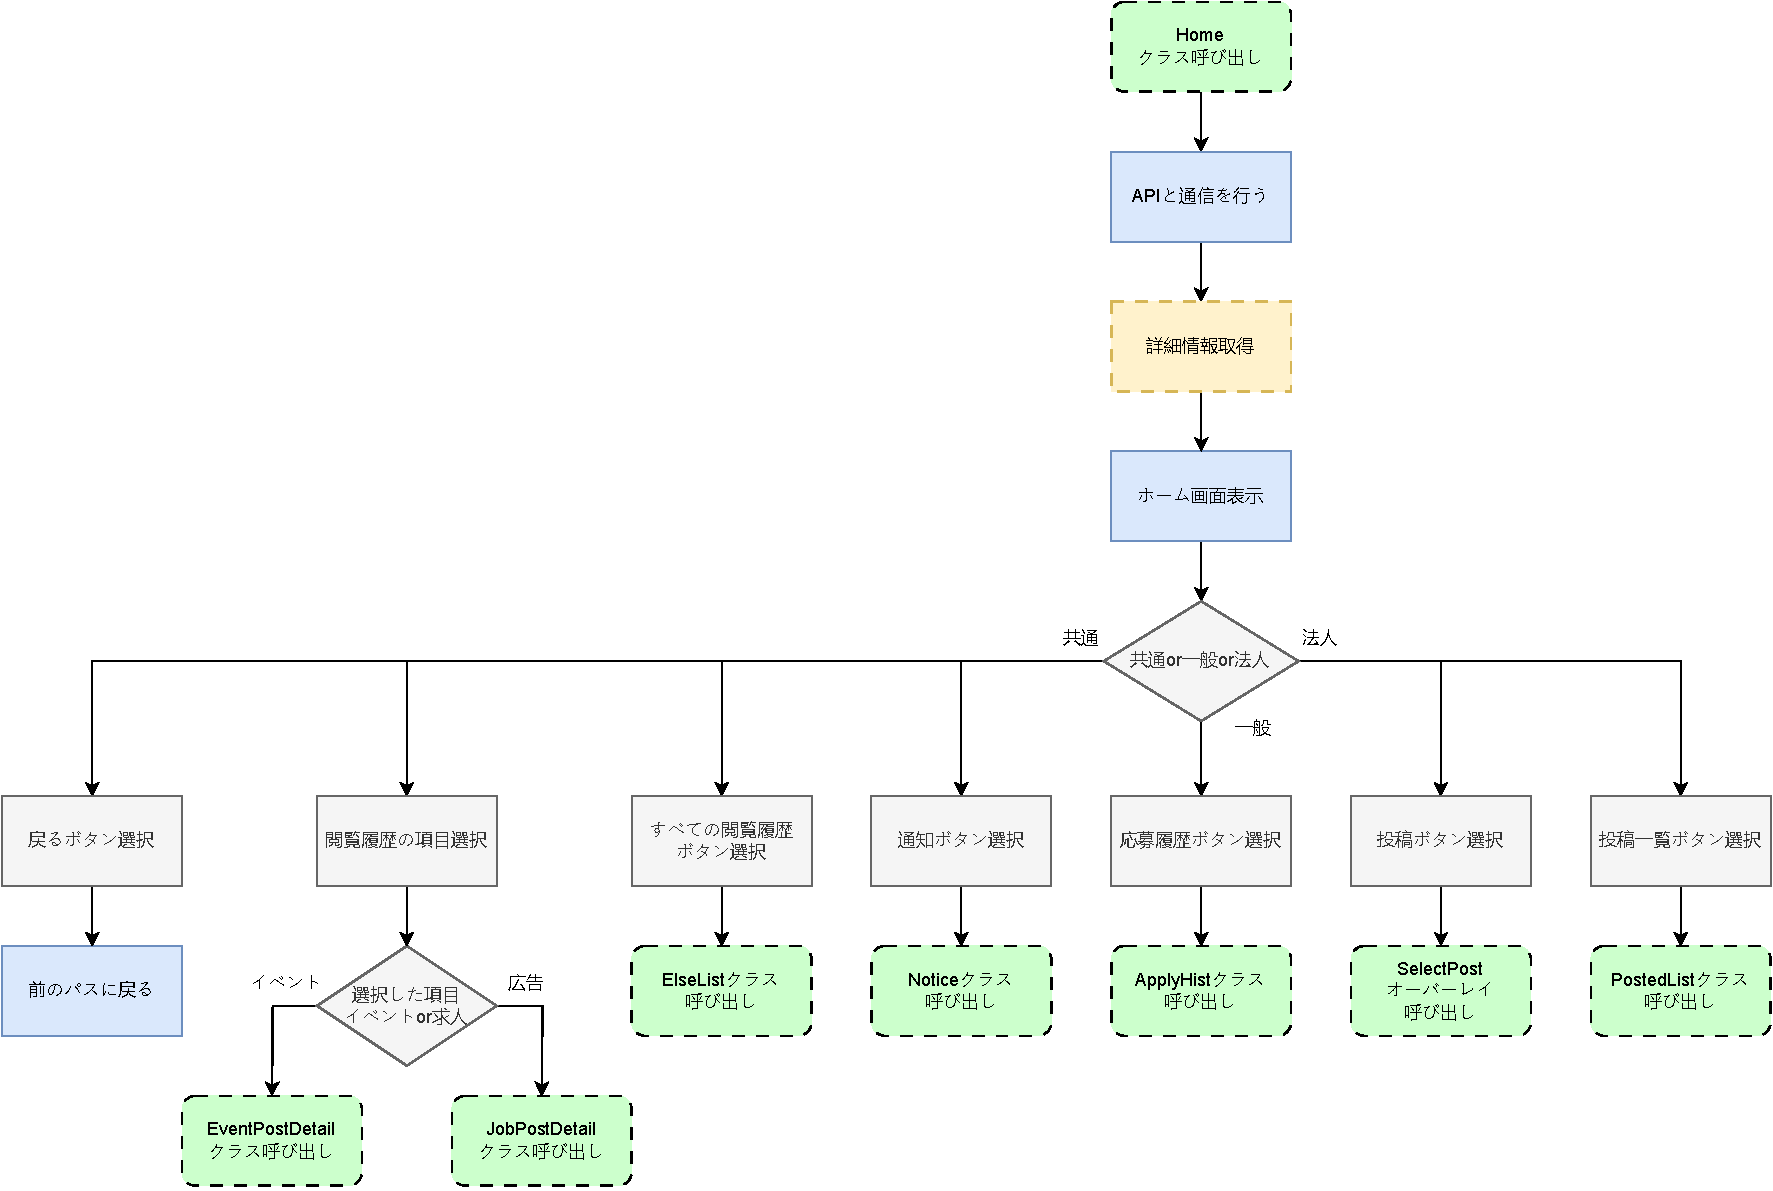
\includegraphics[width=15cm]{./images/internal-design/state_change_diagram/home/home.pdf}
  \caption{home.dartの状態遷移図}
\end{figure}

\begin{table}[H]
  \centering
  \begin{tabular}{|c|l|l|} \hline
    モジュール名                & \multicolumn{2}{l|}{notice.dart}                                                                                                               \\ \hline
    モジュール概要               & \multicolumn{2}{p{12cm}|}{通知画面を作成するモジュール}                                                                                                      \\ \hline
    責任者                   & \multicolumn{2}{l|}{新谷光城}                                                                                                                      \\ \hline
    \multirow{7}{*}{構成要素} & クラス名                                                       & Notice                                                                            \\ \cline{2-3}
                          & クラス種類                                                      & extends StatelessWidget                                                           \\ \cline{2-3}
                          & 処理概要                                                       & \multicolumn{1}{p{12cm}|}{通知画面のWidgetを動的に変更するクラス}                                 \\ \cline{2-3}
                          & 入力                                                         & なし                                                                                \\ \cline{2-3}
                          & 出力                                                         & Widget                                                                            \\ \cline{2-3}
                          & \multicolumn{2}{l|}{他クラス・関数との関係}                                                                                                               \\ \cline{2-3}
                          & \multicolumn{2}{p{14cm}|}{notice.dartのNoticeStateクラスを組み込む}                                                                                     \\ \hline
    \multirow{7}{*}{構成要素} & クラス名                                                       & NoticeState                                                                       \\ \cline{2-3}
                          & クラス種類                                                      & extends StatelessWidget                                                           \\ \cline{2-3}
                          & 処理概要                                                       & \multicolumn{1}{p{12cm}|}{通知画面の状態を返すクラス}                                          \\ \cline{2-3}
                          & 入力                                                         & なし                                                                                \\ \cline{2-3}
                          & 出力                                                         & State                                                                             \\ \cline{2-3}
                          & \multicolumn{2}{l|}{他クラス・関数との関係}                                                                                                               \\ \cline{2-3}
                          & \multicolumn{2}{p{14cm}|}{
      notice.dartのNoticeListViewクラスを組み込む
      \newline change\_general\_corporation.dartのChangeGeneralCorporationプロバイダを組み込む
      \newline title\_appbar.dartのTitleAppBarクラスを組み込む
    \newline toggle\_button.dartのToggleButtonクラスを組み込む}                                                                                                                     \\ \hline
    \multirow{7}{*}{構成要素} & クラス名                                                       & NoticeListView                                                                    \\ \cline{2-3}
                          & クラス種類                                                      & extends StatelessWidget                                                           \\ \cline{2-3}
                          & 処理概要                                                       & \multicolumn{1}{p{12cm}|}{通知の一覧を生成するクラス}                                          \\ \cline{2-3}
                          & 入力                                                         & bool is\_event, List$<$List$<$Map$<$String, dynamic$>$$>$$>$ items, String detail \\ \cline{2-3}
                          & 出力                                                         & Widget                                                                            \\ \cline{2-3}
                          & \multicolumn{2}{l|}{他クラス・関数との関係}                                                                                                               \\ \cline{2-3}
                          & \multicolumn{2}{p{14cm}|}{
      change\_general\_corporation.dartのChangeGeneralCorporationプロバイダを組み込む
      \newline notice\_detail.dartのNoticeDetailクラスを呼び出すことで通知詳細画面を表示
    \newline 戻るボタンの選択で前のモジュールに戻る}                                                                                                                                          \\ \hline
  \end{tabular}
\end{table}

\begin{figure}[H]
  \centering
  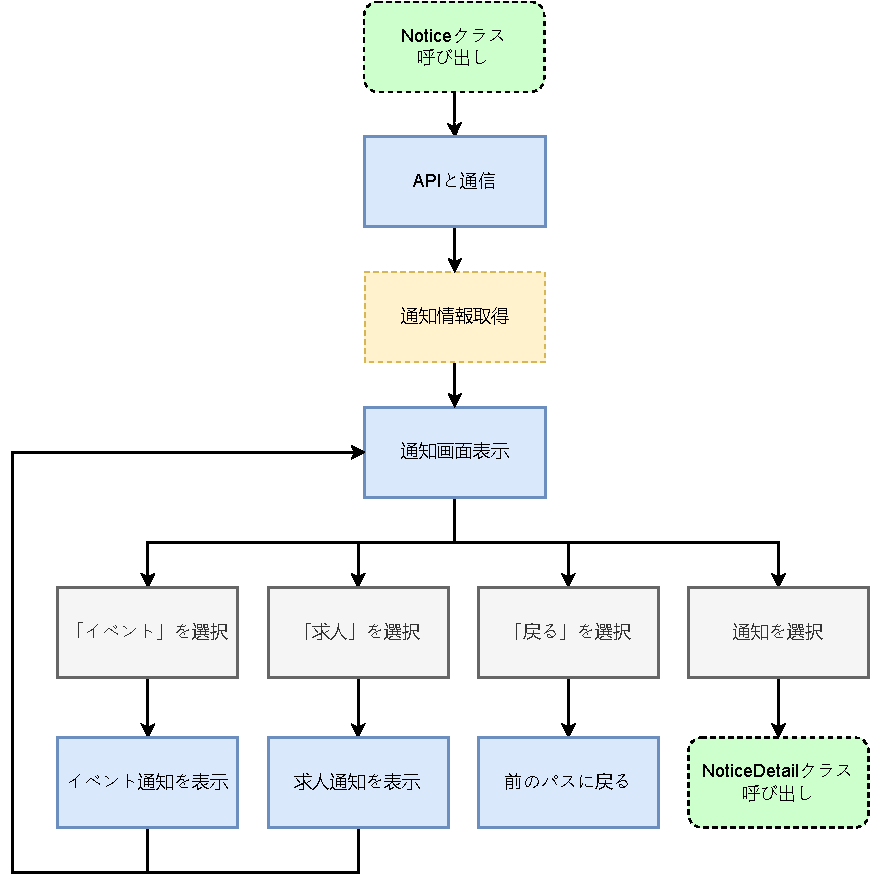
\includegraphics[scale = 0.9]{./images/internal-design/state_change_diagram/home/notice.pdf}
  \caption{notice.dartの状態遷移図}
\end{figure}

\begin{table}[H]
  \centering
  \begin{tabular}{|c|l|l|} \hline
    モジュール名                & \multicolumn{2}{l|}{notice\_detail.dart}                                                                                                                               \\ \hline
    モジュール概要               & \multicolumn{2}{p{12cm}|}{通知の詳細画面を表示するモジュール}                                                                                                                           \\ \hline
    責任者                   & \multicolumn{2}{l|}{新谷光城}                                                                                                                                              \\ \hline
    \multirow{7}{*}{構成要素} & クラス名                                         & NoticeDetail                                                                                                            \\ \cline{2-3}
                          & クラス種類                                        & extends StatelessWidget                                                                                                 \\ \cline{2-3}
                          & 処理概要                                         & \multicolumn{1}{p{12cm}|}{任意の通知詳細画面を生成するクラス}                                                                            \\ \cline{2-3}
                          & 入力                                           & \multicolumn{1}{p{12cm}|}{List$<$List$<$Map$<$String, dynamic$>$$>$$>$ titles, int is\_event, int index, String detail} \\ \cline{2-3}
                          & 出力                                           & Widget                                                                                                                  \\ \cline{2-3}
                          & \multicolumn{2}{l|}{他クラス・関数との関係}                                                                                                                                       \\ \cline{2-3}
                          & \multicolumn{2}{p{14cm}|}{
      titleAppBar.dartのTitleAppBarクラスを組み込む
      \newline noticeDetail.dartのNoticeContentクラスを組みむ
    \newline 戻るボタンの選択で前のモジュールに戻る}                                                                                                                                                                  \\ \hline
    \multirow{7}{*}{構成要素} & クラス名                                         & NoticeContent                                                                                                           \\ \cline{2-3}
                          & クラス種類                                        & extends StatelessWidget                                                                                                 \\ \cline{2-3}
                          & 処理概要                                         & \multicolumn{1}{p{12cm}|}{任意の通知内容のタイトルと本文を生成するクラス}                                                                      \\ \cline{2-3}
                          & 入力                                           & String title, String detail                                                                                             \\ \cline{2-3}
                          & 出力                                           & Widget                                                                                                                  \\ \cline{2-3}
                          & \multicolumn{2}{l|}{他クラス・関数との関係}                                                                                                                                       \\ \cline{2-3}
                          & \multicolumn{2}{p{14cm}|}{なし}                                                                                                                                          \\ \hline
  \end{tabular}
\end{table}

\begin{figure}[H]
  \centering
  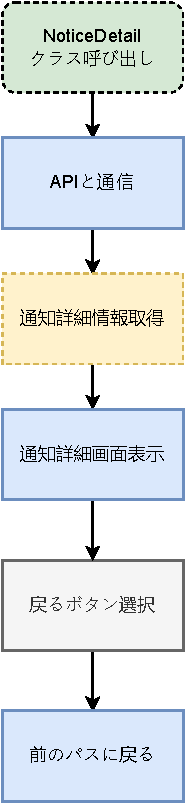
\includegraphics[scale = 0.9]{./images/internal-design/state_change_diagram/home/notice_detail.pdf}
  \caption{notice\_detail.dartの状態遷移図}
\end{figure}

\begin{table}[H]
  \centering
  \begin{tabular}{|c|l|l|} \hline
    モジュール名                & \multicolumn{2}{l|}{apply\_hist.dart}                                                            \\ \hline
    モジュール概要               & \multicolumn{2}{p{12cm}|}{応募を行った求人広告一覧を表示するモジュール}                                                \\ \hline
    責任者                   & \multicolumn{2}{l|}{新谷光城}                                                                        \\ \hline
    \multirow{7}{*}{構成要素} & クラス名                                              & ApplyHist                                    \\ \cline{2-3}
                          & クラス種類                                             & extends StatelessWidget                      \\ \cline{2-3}
                          & 処理概要                                              & \multicolumn{1}{p{12cm}|}{応募一覧画面を動的に変更するクラス} \\ \cline{2-3}
                          & 入力                                                & なし                                           \\ \cline{2-3}
                          & 出力                                                & Widget                                       \\ \cline{2-3}
                          & \multicolumn{2}{l|}{他クラス・関数との関係}                                                                 \\ \cline{2-3}
                          & \multicolumn{2}{p{14cm}|}{ApplyHistStateクラスを組み込む}                                                \\ \hline
    \multirow{7}{*}{構成要素} & クラス名                                              & ApplyHistState                               \\ \cline{2-3}
                          & クラス種類                                             & extends StatelessWidget                      \\ \cline{2-3}
                          & 処理概要                                              & \multicolumn{1}{p{12cm}|}{応募一覧画面の状態を返すクラス}   \\ \cline{2-3}
                          & 入力                                                & なし                                           \\ \cline{2-3}
                          & 出力                                                & State                                        \\ \cline{2-3}
                          & \multicolumn{2}{l|}{他クラス・関数との関係}                                                                 \\ \cline{2-3}
                          & \multicolumn{2}{p{14cm}|}{
      title\_appbar.dartのTitleAppBarクラスを組み込む
      \newline post\_list.dartのPostListクラスを組み込む
    \newline 戻るボタンの選択で前のモジュールに戻る}                                                                                            \\ \hline
  \end{tabular}
\end{table}

\begin{figure}[H]
  \centering
  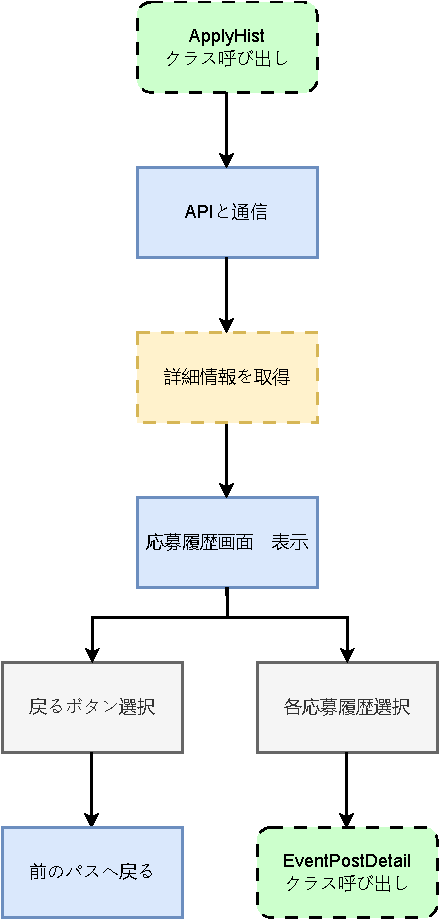
\includegraphics[scale = 0.8]{./images/internal-design/state_change_diagram/home/apply_hist.pdf}
  \caption{apply\_hist.dartの状態遷移図}
\end{figure}